\chapter{Dispiegamento in opera}

\section{Architettura di deployment}

Il deployment delle landing pages Next.js è stato progettato secondo 
un'architettura cloud-native basata su container Docker (tecnologia che 
impacchetta l'applicazione e tutte le sue dipendenze in unità isolate 
chiamate container) e infrastruttura AWS.

\subsection{Stack deployment}

L'applicazione è stata deployata su infrastruttura AWS con approccio cloud-native. 
La scelta di AWS è coerente con l'infrastruttura già presente per gli altri 
prodotti aziendali (backend Django, database PostgreSQL), permettendo di 
riutilizzare competenze DevOps del team e mantenere consistenza architetturale.

La strategia di rendering ha combinato Static Site Generation per contenuti statici 
come le landing principali, con Incremental Static Regeneration e revalidation 
ogni ora per i contenuti dinamici. Questo approccio ibrido garantisce tempi di 
caricamento ottimali attraverso HTML pre-generato, mantenendo al contempo i 
contenuti aggiornati senza necessità di rebuild completi dell'applicazione.

La containerizzazione Docker adotta build multi-stage (processo in più fasi 
che separa compilazione e runtime per ridurre le dimensioni finali dell'immagine) 
per ottimizzazione delle dimensioni delle immagini finali. Le immagini Docker 
vengono gestite tramite AWS Elastic Container Registry (ECR, registro per 
archiviare e gestire immagini Docker) nella region eu-south-1, con repository 
separati per staging e production. Gli asset statici (immagini, CSS, JavaScript) 
sono salvati sul servizio di storage AWS S3 (Simple Storage Service) per 
gestione efficiente e caching distribuito tramite CloudFront, Content Delivery 
Network (CDN) globale di AWS.

\section{Processo deployment}

Il deployment è gestito attraverso script bash automatizzati che orchestrano 
l'intero processo di rilascio, coinvolgendo diversi attori e sistemi per 
garantire rilasci sicuri e consistenti.

\subsection{Pipeline di rilascio}

Il workflow prevede una serie di passaggi sequenziali con validazione automatica 
a ogni step:

\begin{enumerate}
  \item \textbf{Autenticazione}: login su AWS ECR tramite AWS CLI per autorizzare 
        push delle immagini Docker.
  \item \textbf{Validazione codice}: type checking TypeScript (\texttt{pnpm ts-check}) 
        e linting ESLint (\texttt{pnpm lint}) per applicare gli standard di codifica del team.
  \item \textbf{Build immagine}: compilazione immagine Docker con variabili 
        ambiente specifiche per staging o production.
  \item \textbf{Tag e versionamento}: applicazione tag all'immagine seguendo 
        la nomenclatura repository ECR.
  \item \textbf{Push registry}: upload dell'immagine su AWS ECR nella regione eu-south-1.
\end{enumerate}

\medskip
Questo processo strutturato garantisce validazione automatica del codice prima 
di ogni deployment, riducendo il rischio di regressioni in produzione. La Figura 
\ref{fig:deployment-pipeline} illustra il flusso completo dal codice locale fino 
agli utenti finali, evidenziando gli attori coinvolti e i checkpoint di validazione 
tra i diversi ambienti.

\begin{figure}[h!]
    \centering
    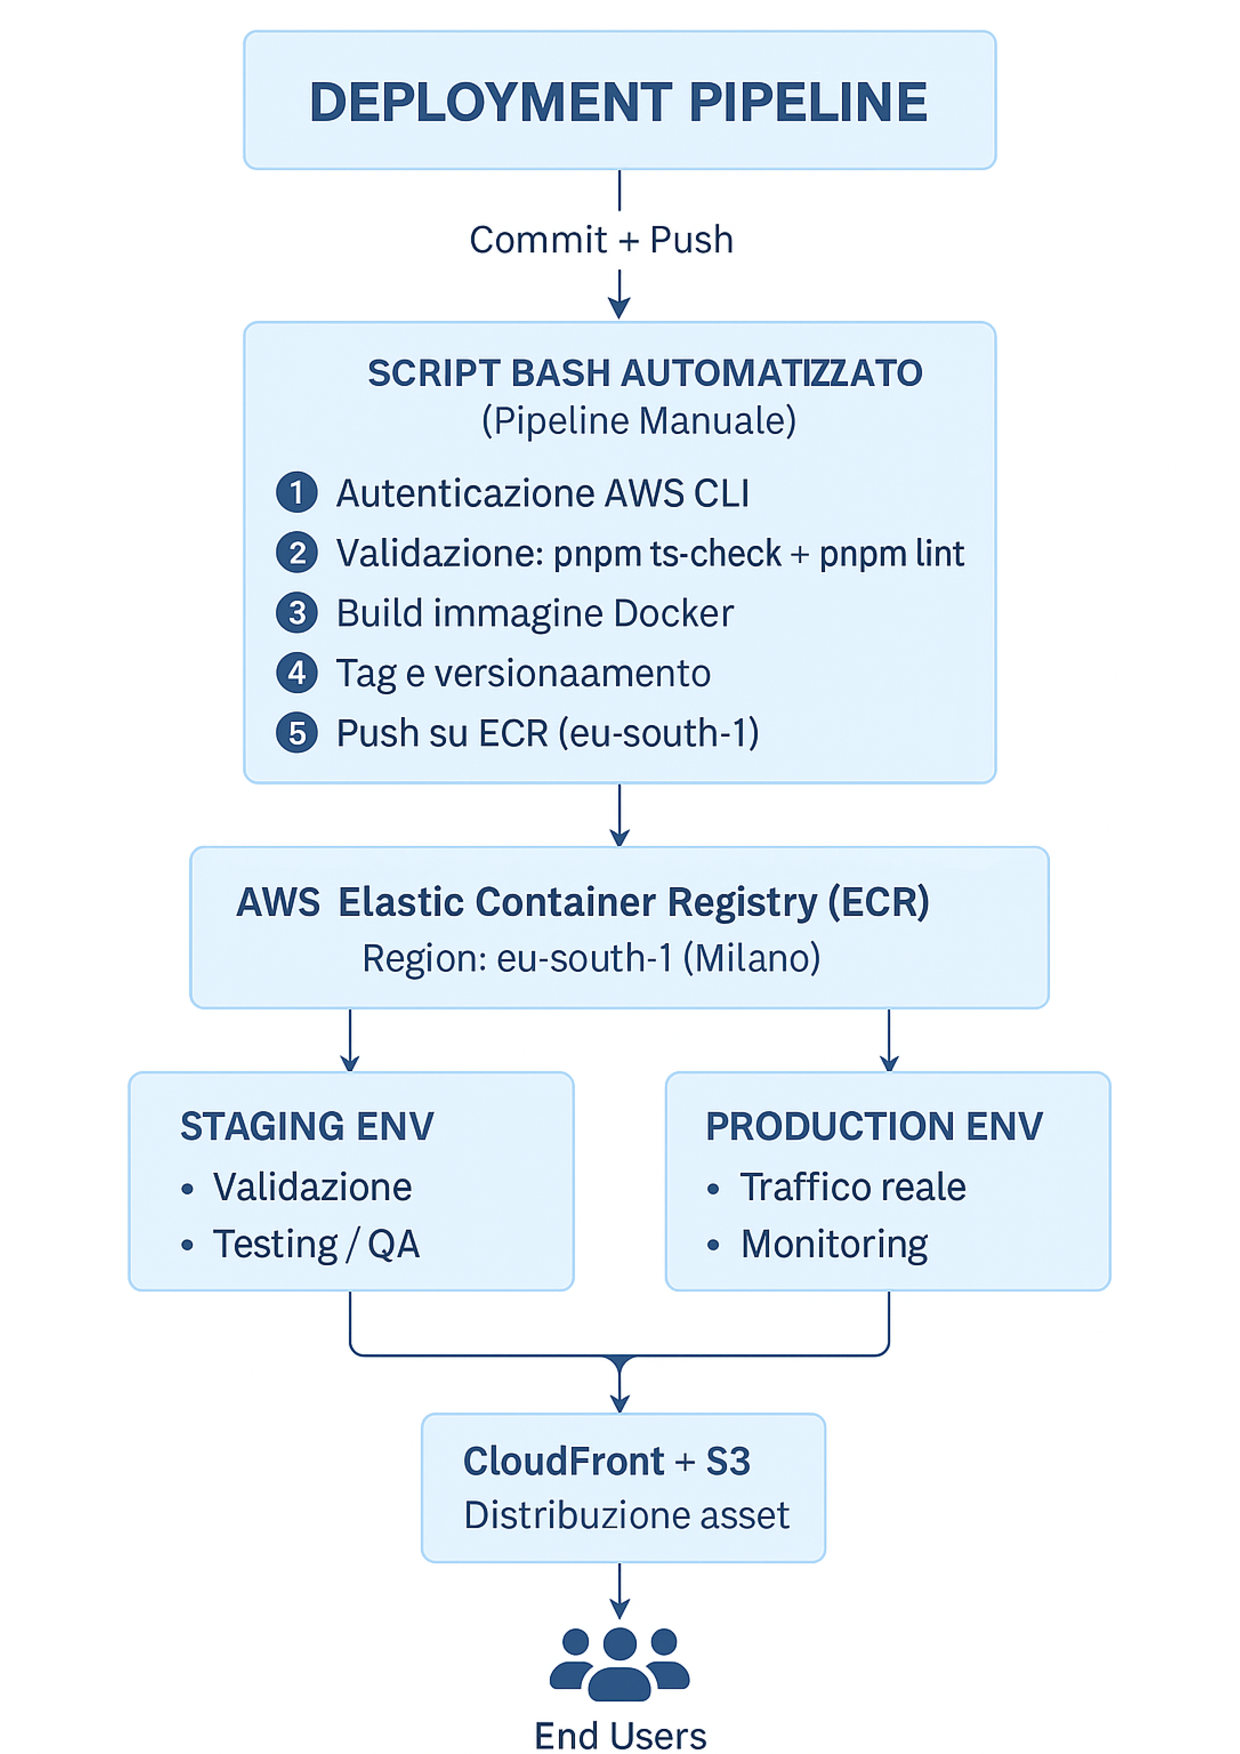
\includegraphics[width=0.9\textwidth]{chapters/figures/aws.pdf}
    \caption{Pipeline di deployment con attori coinvolti e flusso di rilascio 
    attraverso gli ambienti staging e production.}
    \label{fig:deployment-pipeline}
\end{figure}
\clearpage

\subsection{Gestione ambienti}

L'infrastruttura prevede tre ambienti separati con configurazioni dedicate, 
come illustrato nella pipeline. L'\textbf{ambiente Development} locale utilizza 
file di configurazione specifici per sviluppo, permettendo ai developer di testare 
modifiche senza impattare altri ambienti. L'\textbf{ambiente Staging} con repository 
ECR dedicato permette testing e validazione delle release prima del go-live. 
L'\textbf{ambiente Production} con repository ECR dedicato serve il traffico 
reale degli utenti finali.

Questa separazione rigorosa previene deploy accidentali in production e permette 
validazione approfondita delle modifiche. La configurazione ambiente viene caricata 
dinamicamente all'avvio del container tramite merge di file base con file specifico 
per ambiente, separando codice applicativo da configurazioni.

\section{Ottimizzazioni rendering}

Le landing pages principali sfruttano un approccio ibrido di rendering basato su 
Static Site Generation per i contenuti statici e Incremental Static Regeneration 
per i contenuti dinamici, con rigenerazione automatica ogni ora. Questo modello 
consente di garantire tempi di caricamento ottimali e aggiornamenti periodici 
senza dover eseguire rebuild completi dell'applicazione.

Un caso applicativo esteso di questa architettura è rappresentato dal 
\textbf{blog tecnico aziendale}, già integrato nella codebase. In questo contesto, 
le pagine vengono generate staticamente e aggiornate tramite revalidation on-demand 
quando vengono pubblicati nuovi articoli. Pur non costituendo il focus del progetto, 
questa implementazione ha permesso di validare la scalabilità del sistema di 
rendering e la gestione automatica dei contenuti dinamici.

Il componente \texttt{next/image} ottimizza automaticamente le immagini con 
caricamento differito (lazy loading), conversione in formato WebP per browser 
moderni e generazione di versioni responsive, garantendo performance elevate 
e qualità visiva su tutti i dispositivi.

\section{Gestione contenuti e internazionalizzazione}

L'architettura di deployment integra un'area amministrativa preesistente per 
la gestione del blog tecnico aziendale, che utilizza lo stesso sistema di 
revalidation on-demand delle landing pages. Questa integrazione dimostra la 
scalabilità del sistema di rendering adottato.

Il sistema di \textbf{internazionalizzazione} supporta italiano e inglese con 
generazione automatica di route statiche per entrambe le lingue. Le traduzioni 
sono centralizzate in file JSON per ogni locale, semplificando gli aggiornamenti. 
Il rilevamento automatico della lingua dall'header HTTP del browser reindirizza 
gli utenti alla versione più appropriata del sito.

\section{Risultati deployment}

L'architettura di deployment ha garantito rilasci consistenti cross-ambiente grazie 
a Docker multi-stage, separazione chiara degli ambienti staging e production su ECR, 
e validazione automatica pre-deploy tramite TypeScript type checking ed ESLint. 
La gestione efficiente degli asset statici con S3 e la flessibilità nella gestione 
contenuti con area amministrativa integrata forniscono una base scalabile 
per l'ecosistema delle landing pages.

\bigskip
L'infrastruttura fornisce una base solida orientata a developer experience 
grazie all'uso di \texttt{pnpm} e alla configurazione \texttt{TypeScript strict}, 
e performance rendering tramite Static Site Generation e Incremental Static 
Regeneration. L'implementazione futura di pipeline CI/CD (Continuous Integration/
Continuous Deployment, automazione completa del processo di test e rilascio) 
completamente automatizzata, prevista in roadmap aziendale, consentirà di 
aumentare ulteriormente la frequenza dei rilasci e ridurre il time-to-market.